% Beamer presentation for the RL project
\documentclass[aspectratio=169]{beamer}

\usetheme{Madrid}
\usecolortheme{seahorse}
% Eliminăm barele de navigare (sus/jos) de pe toate slide-urile
\setbeamertemplate{navigation symbols}{}
\setbeamertemplate{headline}{}
\setbeamertemplate{footline}{}

\usepackage[T1]{fontenc}
\usepackage[utf8]{inputenc}
\usepackage{amsmath, amssymb}
\usepackage{graphicx}
\usepackage{booktabs}
\usepackage{tikz}
\usetikzlibrary{arrows.meta, positioning, shapes.geometric}

% Diagram macros (inline for portability)
\newcommand{\RLLoopDiagramSmall}{%
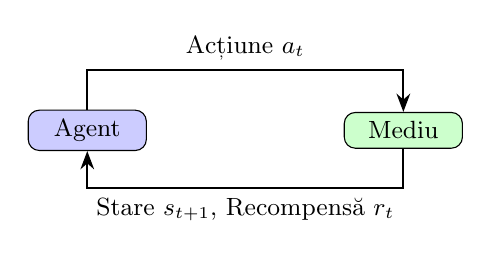
\begin{tikzpicture}[>=Stealth, node distance=2cm, every node/.style={font=\small}]
  \node[draw, rounded corners, fill=blue!20, minimum width=1.5cm] (agent) {Agent};
  \node[draw, rounded corners, fill=green!20, minimum width=1.5cm, right=2.5cm of agent] (env) {Mediu};
  \draw[->, thick] (agent.north) -- ++(0,0.5) -| node[above, pos=0.25]{Acțiune $a_t$} (env.north);
  \draw[->, thick] (env.south) -- ++(0,-0.5) -| node[below, pos=0.25]{Stare $s_{t+1}$, Recompensă $r_t$} (agent.south);
\end{tikzpicture}
}

\title{RL pentru conducere autonomă într-un mediu personalizat ``Highway''}
\subtitle{Mediu personalizat ``Highway''}
\author{Echipa Juno: \and Corobana Ingrid, Moise Irina, Prizlopan Iustin, Sescu Matei}
\institute{Universitatea din București}
\date{Ianuarie 2026}

\begin{document}

% ============== SLIDE 1 ==============
\begin{frame}
  \titlepage
\end{frame}

% ============== SLIDE 2 ==============
\begin{frame}{Problema și obiectivul}
  \begin{columns}
    \begin{column}{0.55\textwidth}
      \textbf{Scop:} Antrenarea unui agent care să conducă un vehicul (mașina galbenă) într-un mediu de trafic cu mai multe benzi.
      
      \vspace{0.3cm}
      \textbf{Cerințe:}
      \begin{itemize}
        \item Să evite coliziunile cu mașinile albastre
        \item Să rămână pe carosabil
        \item Să mențină o viteză rezonabilă
      \end{itemize}
      
      \vspace{0.3cm}
      \textbf{Abordare:} Reinforcement Learning — agentul învață din recompense, fără supervizare explicită.
    \end{column}
    \begin{column}{0.4\textwidth}
      \centering
      \RLLoopDiagramSmall
      
      \vspace{0.3cm}
      {\footnotesize Schema agent–mediu}
    \end{column}
  \end{columns}
\end{frame}

% ============== SLIDE 3 ==============
\begin{frame}{Stare, Acțiune, Recompensă}
  \begin{block}{Stare (observație)}
    Vector continuu de 25 dimensiuni: poziția, viteza și orientarea vehiculului ego + informații despre vehiculele din jur.
  \end{block}
  
  \begin{block}{Acțiuni (discrete)}
    \begin{tabular}{cl}
      0 & Idle (nu face nimic) \\
      1 & Accelerează \\
      2 & Frânează \\
      3 & Virează stânga \\
      4 & Virează dreapta \\
    \end{tabular}
  \end{block}
  
  \begin{block}{Recompensă}
    \textcolor{red}{$-1$} coliziune/ieșire drum \quad \textcolor{green!60!black}{$+1$} viteză (aliniată bandă) / centru bandă
  \end{block}
\end{frame}

% ============== SLIDE 4 ==============
\begin{frame}{Designul mediului (environment)}
  \begin{columns}
    \begin{column}{0.5\textwidth}
      \textbf{Drum personalizat:}
      \begin{itemize}
        \item Segment drept de intrare
        \item Zonă de îmbinare (merge)
        \item Viraj circular
        \item Porțiuni drepte
        \item Ieșire verticală
      \end{itemize}
      
      \vspace{0.3cm}
      \textbf{Vehicule:}
      \begin{itemize}
        \item \textcolor{yellow!80!black}{Ego} = mașina controlată
        \item \textcolor{blue}{Trafic} = mașini IDM (model de conducere realist)
      \end{itemize}
    \end{column}
    \begin{column}{0.45\textwidth}
      \centering
      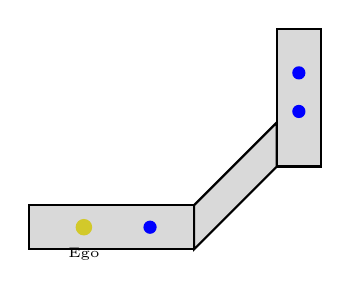
\begin{tikzpicture}[scale=0.7]
        % Road segments
        \draw[thick, fill=gray!30] (0,0) rectangle (3,0.8);
        \draw[thick, fill=gray!30] (3,0) -- (4.5,1.5) -- (4.5,2.3) -- (3,0.8) -- cycle;
        \draw[thick, fill=gray!30] (4.5,1.5) rectangle (4.5+0.8,4);
        % Ego car
        \fill[yellow!80!black] (1,0.4) circle (0.15);
        \node[below, font=\tiny] at (1,0.2) {Ego};
        % Traffic
        \fill[blue] (2.2,0.4) circle (0.12);
        \fill[blue] (4.9,2.5) circle (0.12);
        \fill[blue] (4.9,3.2) circle (0.12);
      \end{tikzpicture}
      
      {\footnotesize Schemă simplificată a drumului}
    \end{column}
  \end{columns}
\end{frame}

% ============== SLIDE 5 ==============
\begin{frame}{Algoritmi implementați}
  \begin{columns}[T]
    \begin{column}{0.32\textwidth}
      \begin{block}{\centering Tabular Q-Learning}
        \begin{itemize}
          \item Stare discretizată (6 dim)
          \item Tabel Q de 1944 stări
          \item Update Bellman clasic
          \item $\varepsilon$-greedy
        \end{itemize}
      \end{block}
    \end{column}
    
    \begin{column}{0.32\textwidth}
      \begin{block}{\centering DQN}
        \begin{itemize}
          \item Stare continuă (25 dim)
          \item Rețea: 256→128→5
          \item Experience Replay
          \item Target Network
          \item Double DQN
        \end{itemize}
      \end{block}
    \end{column}
    
    \begin{column}{0.32\textwidth}
      \begin{block}{\centering REINFORCE + Baseline}
        \begin{itemize}
          \item Policy network
          \item Value network
          \item Monte Carlo returns
          \item Advantage $A_t = G_t - V(s_t)$
        \end{itemize}
      \end{block}
    \end{column}
  \end{columns}
  
  \vspace{0.5cm}
  \centering
  \textbf{Toți agenții} folosesc aceleași 5 acțiuni discrete și același mediu.
\end{frame}

% ============== SLIDE 6 ==============
\begin{frame}{Curbe de antrenare}
  \centering
  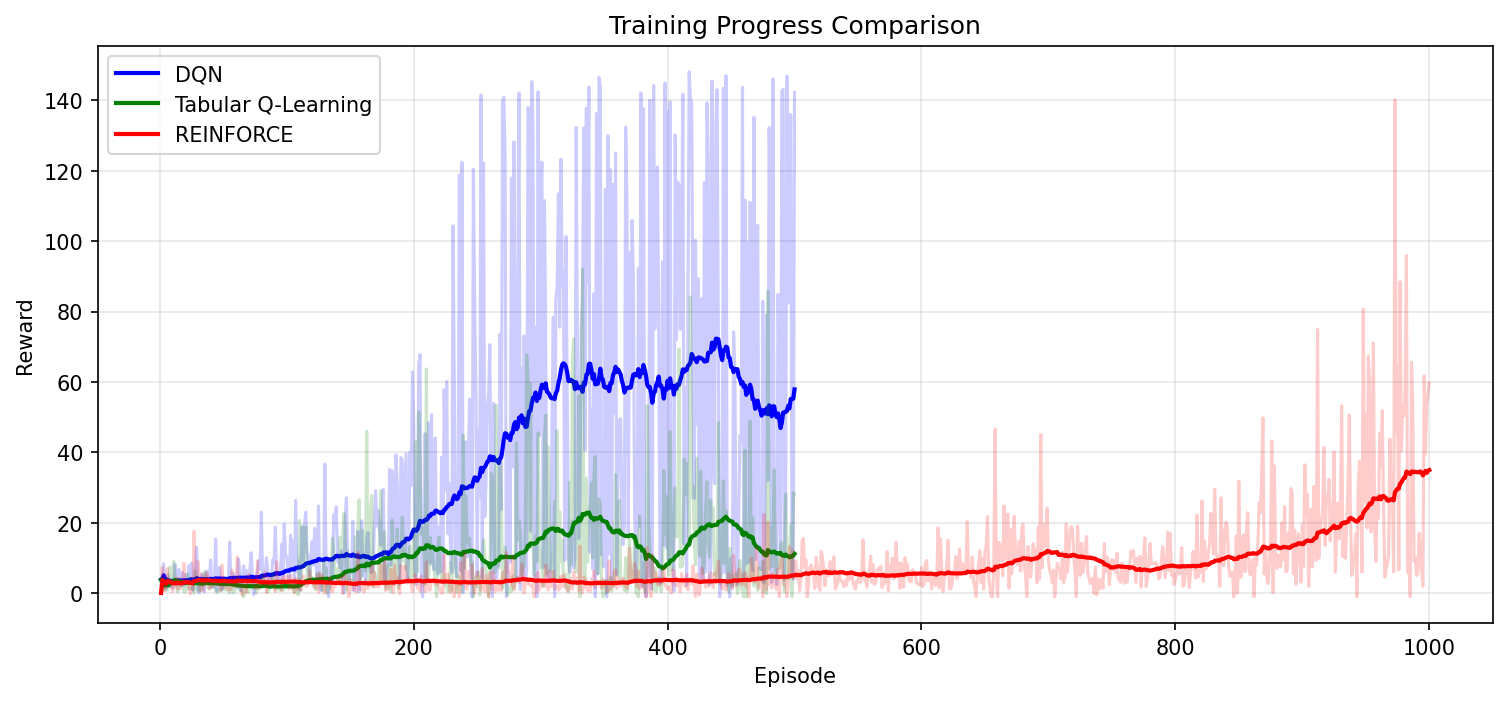
\includegraphics[width=0.85\textwidth]{../results/training_comparison.png}
  
  \vspace{0.3cm}
  {\small DQN converge cel mai rapid și atinge recompense mai mari. REINFORCE este mai instabil. Tabular învață mai lent.}
\end{frame}

% ============== SLIDE 7 ==============
\begin{frame}{Vizualizarea comportamentului}
  \begin{columns}
    \begin{column}{0.33\textwidth}
      \centering
      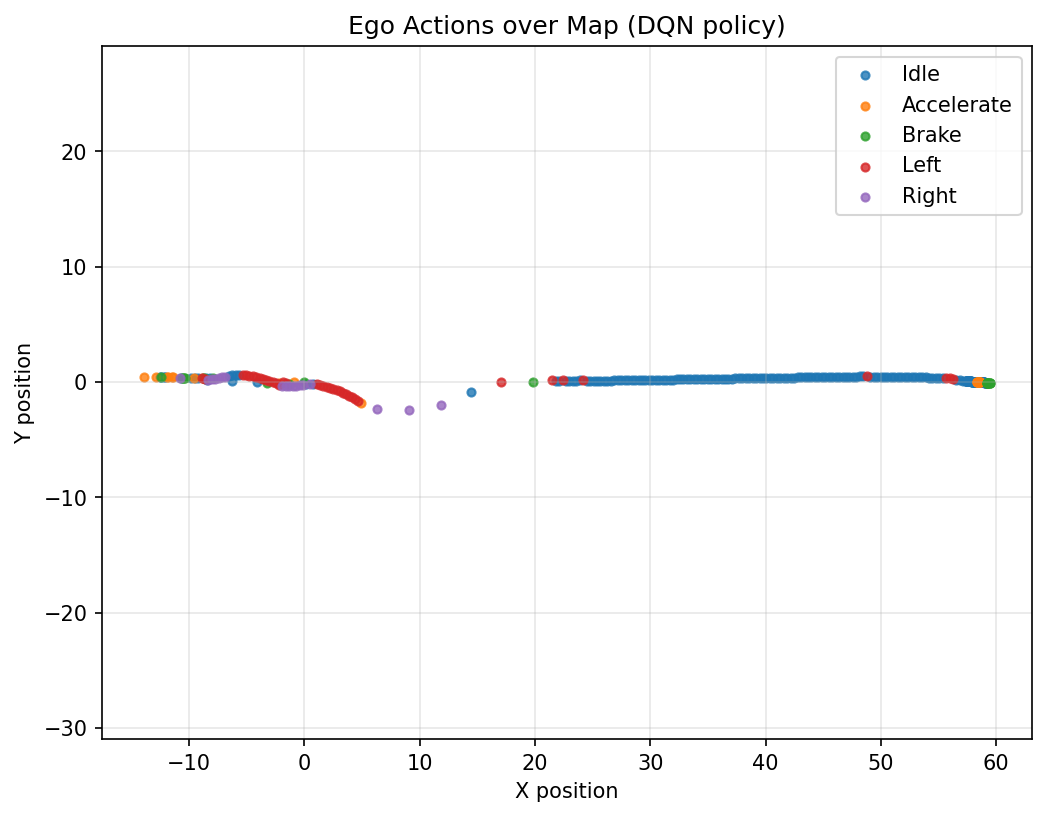
\includegraphics[width=\textwidth]{../results/actions_dqn.png}
      {\footnotesize DQN}
    \end{column}
    \begin{column}{0.33\textwidth}
      \centering
      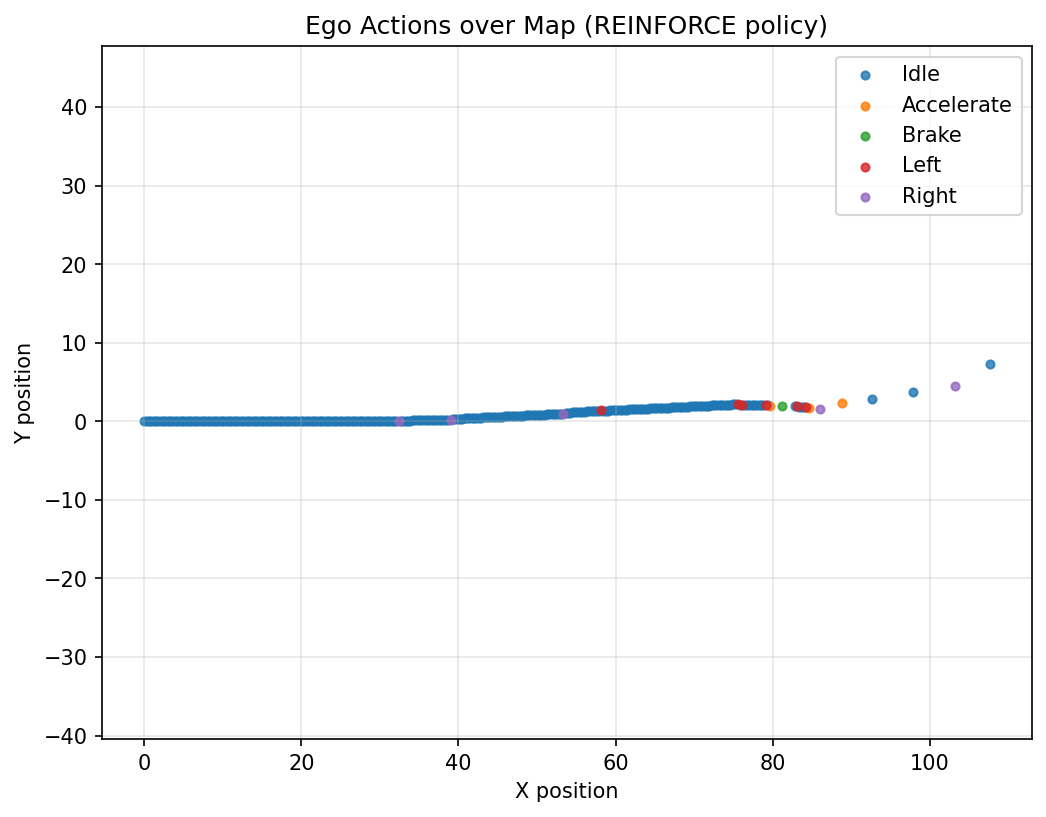
\includegraphics[width=\textwidth]{../results/actions_reinforce.png}
      {\footnotesize REINFORCE}
    \end{column}
    \begin{column}{0.33\textwidth}
      \centering
      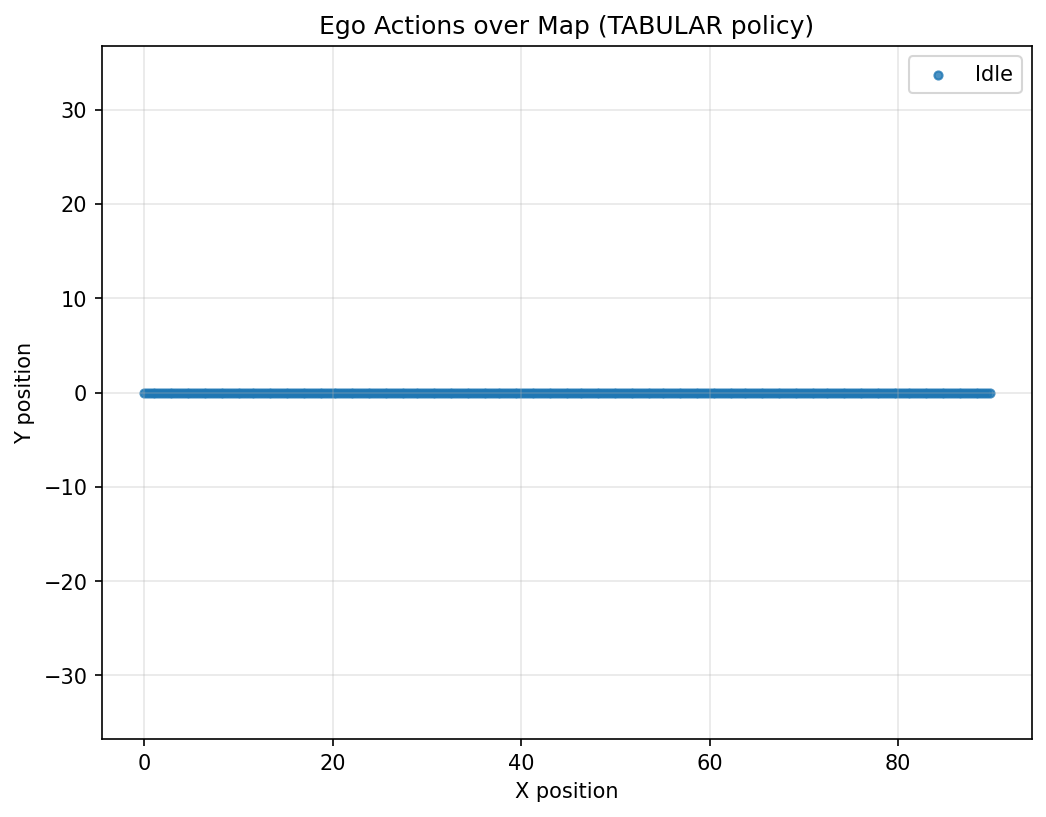
\includegraphics[width=\textwidth]{../results/actions_tabular.png}
      {\footnotesize Tabular}
    \end{column}
  \end{columns}
  
  \vspace{0.3cm}
  \begin{itemize}
    \item Culorile indică acțiunile alese în fiecare poziție
    \item DQN: traiectorie fluidă, schimbări de bandă planificate
    \item Tabular: decizii mai „rigide" din cauza discretizării
  \end{itemize}
\end{frame}

% ============== SLIDE 8 ==============
\begin{frame}{Evaluare și comparație}
  \begin{columns}
    \begin{column}{0.55\textwidth}
      \centering
      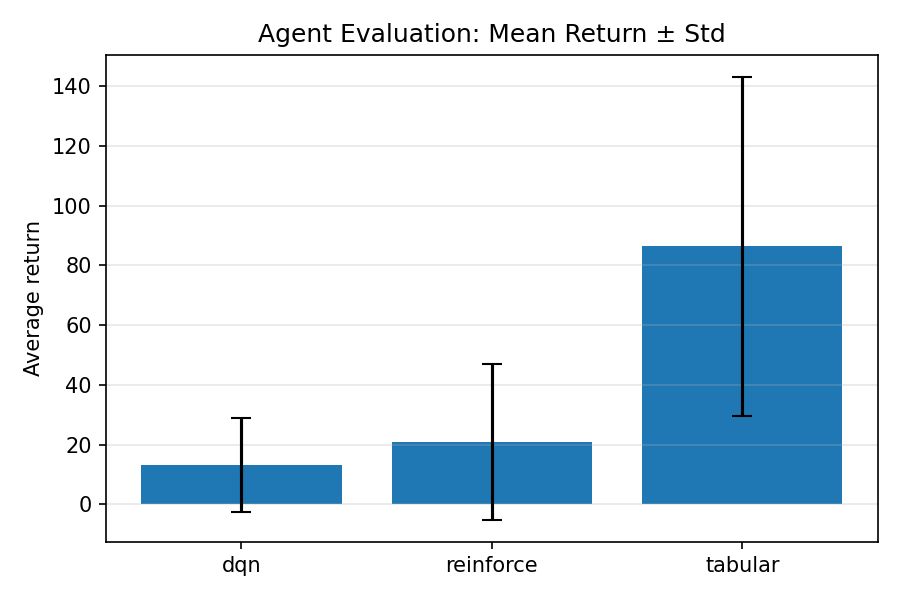
\includegraphics[width=\textwidth]{../results/comparison/eval_barplot.png}
    \end{column}
    \begin{column}{0.4\textwidth}
      \textbf{Ce arată graficul:}
      \begin{itemize}
        \item Înălțimea barei = recompensa medie pe 20 episoade de test
        \item Linia de eroare = deviația standard
        \item Cu cât bara e mai înaltă, cu atât agentul e mai bun
      \end{itemize}
      
      \vspace{0.3cm}
      \textbf{Concluzie:}
      
      În general DQN $>$ REINFORCE $>$ Tabular, dar variază în funcție de antrenare.
    \end{column}
  \end{columns}
\end{frame}

% ============== SLIDE 9 ==============
\begin{frame}{Hiperparametri cheie}
  \begin{table}
    \centering
    \begin{tabular}{lcc}
      \toprule
      \textbf{Parametru} & \textbf{DQN} & \textbf{REINFORCE} \\
      \midrule
      Learning rate & $5 \times 10^{-4}$ & $10^{-3}$ \\
      Discount $\gamma$ & 0.99 & 0.99 \\
      Epsilon decay & 0.99 & — \\
      Buffer size & 50,000 & — \\
      Batch size & 64 & — \\
      Hidden layers & {[}256, 128{]} & {[}64{]} \\
      Episoade & 500 & 1000 \\
      \bottomrule
    \end{tabular}
  \end{table}
  
  \vspace{0.3cm}
  \textbf{Ce a ajutat:} reward shaping, Double DQN, value baseline pentru REINFORCE.
  
  \textbf{Ce a fost dificil:} stabilitatea policy gradient, designul recompensei.
\end{frame}

% ============== SLIDE 10 ==============
\begin{frame}{Lecții învățate și direcții viitoare}
  \begin{columns}
    \begin{column}{0.48\textwidth}
      \textbf{Ce a funcționat bine:}
      \begin{itemize}
        \item DQN + stare kinematics (25 dim)
        \item Mediu personalizat highway\_env
        \item Experience replay + target net
        \item Value baseline pentru REINFORCE
      \end{itemize}
    \end{column}
    \begin{column}{0.48\textwidth}
      \textbf{Direcții viitoare:}
      \begin{itemize}
        \item PPO, A2C (algoritmi mai stabili)
        \item Acțiuni continue native
        \item Scenarii mai complexe (intersecții)
        \item Robustețe la zgomot pe observații
      \end{itemize}
    \end{column}
  \end{columns}
  
  \vspace{0.5cm}
  \centering
  \begin{block}{}
    \centering
    Proiectul demonstrează aplicarea practică a conceptelor de RL (Q-Learning, DQN, Policy Gradient) într-un scenariu de conducere autonomă.
  \end{block}
\end{frame}

% ============== SLIDE 11 ==============
\begin{frame}{}
  \centering
  \Huge \textbf{Întrebări?}
  
  \vspace{1cm}
  \large Demo disponibil cu \texttt{python demo\_agent.py}
  
  \vspace{0.5cm}
  \normalsize
  Cod sursă: \texttt{https://github.com/dirgnic/RL\_project}
\end{frame}

\end{document}
